\documentclass{article}
\usepackage{graphicx}
\usepackage[export]{adjustbox}% Required for inserting images
\usepackage{float}
\usepackage{placeins}



\begin{document}
\section{PS01 Answers}
Aryan Goyal

\noindent Student number: 18306046

\section{Question 1}
    
\subsection{Answer 1.1}
In order to find the 90 percent confidence interval, I calculate some descriptive statistics:
\begin{verbatim}
    mean(y) #central tendency, mean
    sd(y)   #Standard deviation to help gauge the spread of the data
    length(y) #to calculate the sample size
\end{verbatim}

Using these functions, I find that the mean = 98.44, 
the standard deviation = 13.09 and the sample size (n) = 25

\noindent
These values are used to calculate the standard error.
The standard error describes how the mean varies from sample to sample

\begin{verbatim}
    standard_error <- sd(y)/sqrt(25) #25 is the sample size
\end{verbatim}

From the above values, we can calculate the 90 percent confidence interval
The confidence interval formula is: mean +- (t-score * (standard error))
\begin{verbatim}
    t_score <- qt(0.95, df=length(y)-1) 
    lower_90_t <- mean(y)-(t_score)*(standard_error) 
    upper_90_t <- mean(y)+(t_score) * (standard_error)
\end{verbatim}
From this, I got the following confidence intervals:

\begin{center} 
Lower interval:93.9599

Upper interval: 102.9201
\end{center}  
Hence, the average student IQ was 98.44, 90 percent CI[93.9599,102.9201]

\subsection{Answer 1.2}

Based on the question, we have to decide the appropriate hypothesis test.
Due to the small sample size, I have chosen the t-test. 
\vspace{0.3cm}

\noindent My hypotheses: 

Null hypothesis: The mean IQ in her school is less than/equal to 100


Alternative hypothesis: the mean IQ in her school is greater than 100

\vspace{0.3cm}
\noindent 
I conduct a one tailed t test as we are interested in finding out if our mean IQ is greater than 100. 

To calculate this in R:
\begin{verbatim}
    test_statistic <- (mean(y)-100)/(sd(y)/sqrt(length(y)))

    P_value <- pt((test_statistic), df = 24, lower.tail = TRUE)    
\end{verbatim}
In order to double check, I use the t-test function in R:
\begin{verbatim}
    t.test(y, mu = 100, alternative = 'less')
\end{verbatim}

From both of these methods, I find that the p-value = 0.2785

This value is greater than our significance level = 0.05 and therefore,
we do not have sufficient evidence to reject the null hypothesis.

We cannot reject the null hypothesis that the mean IQ in her school is less than/equal to 100

\pagebreak
\section{Question 2}

\subsection{Answer 2.1}
I individually plot each relationship among Y, X1, X2 and X3
Next, I display the code from the first 3 graphs from R. The same code was used with the other variables for each graph:
\begin{verbatim}
plot(expenditure$Y,expenditure$X1,
     xlab="Per capita expenditure on shelters/housing assistance in state",
     ylab="Per capita personal income in state",
     main="The Relationship between expenditure on shelters and per capital 
     personal income")
abline(lm(expenditure$X1 ~ expenditure$Y),col='blue',lty='dashed')
cor(expenditure$Y,expenditure$X1)
text(50, 2500,sprintf("Correlation=%s",
    round(cor(expenditure$X1,expenditure$Y),4)))

plot(expenditure$Y,expenditure$X2,
     xlab="Per capita expenditure on shelters/housing assistance in state",
     ylab="”Financially insecure” residents in state per 100,000",
     main="The Relationship between expenditure 
     on shelters and No. of residents that are financially insecure")
abline(lm(expenditure$X2 ~ expenditure$Y),col='blue',lty='dashed')
cor(expenditure$Y,expenditure$X2)
text(50, 450,sprintf("Correlation=%s",          
    round(cor(expenditure$Y,expenditure$X2),4)))

plot(expenditure$Y,expenditure$X3,
     xlab="Per capita expenditure on shelters/housing assistance in state",
     ylab="No. of people per 1000 residing in urban areas in state",
     main="Relationship between expenditure on shelters 
    and no of people per 1000 residing in urban areas")
abline(lm(expenditure$X3 ~ expenditure$Y),col='blue',lty='dashed')
cor(expenditure$Y,expenditure$X3)
text(50, 800,sprintf("Correlation=%s", 
    round(cor(expenditure$Y,expenditure$X3),4)))
\end{verbatim}

\noindent On the basis of the correlation value and line of best fit, I can say that all variables have a positive weak to moderate correlation.

\noindent The strongest positive moderate correlation (0.59) is between X1 (Per capital personal income in state) and X3(Number of people per 1000 residing in urban areas in state)

\noindent Whereas, the weakest positive correlation (0.21) is between X1 (Per capita personal income in state) and X2("Financially insecure" residents in state per 1000)

\begin{figure} 
    \centering
    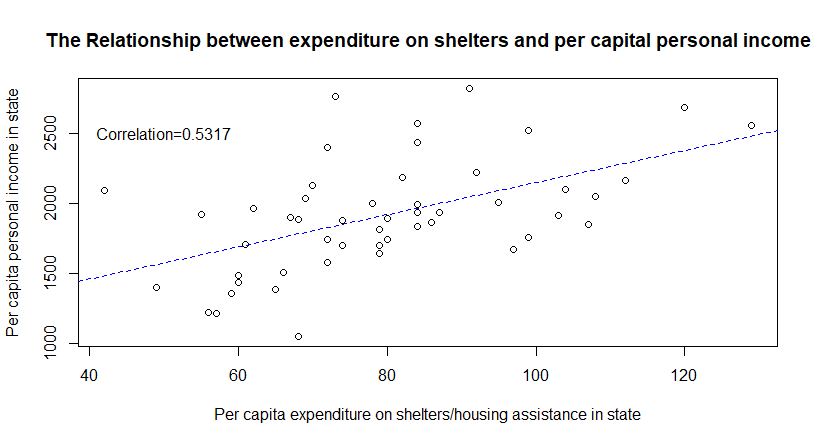
\includegraphics[width=1.3\textwidth]{Y and X1.png}
    \caption{Y and X1}
    \label{fig:enter-label}
\end{figure}

\begin{figure} 
    \centering
    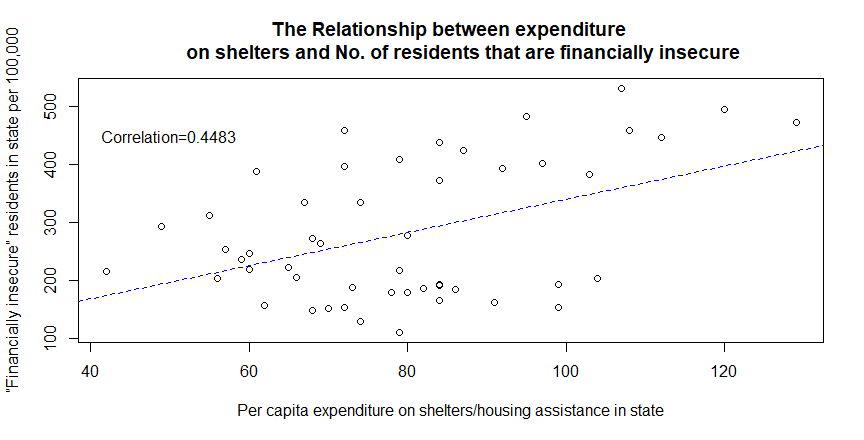
\includegraphics[width=1.3\textwidth]{Y and X2.png}
    \caption{Y and X2}
    \label{fig:enter-label}
\end{figure}

\begin{figure} 
    \centering
    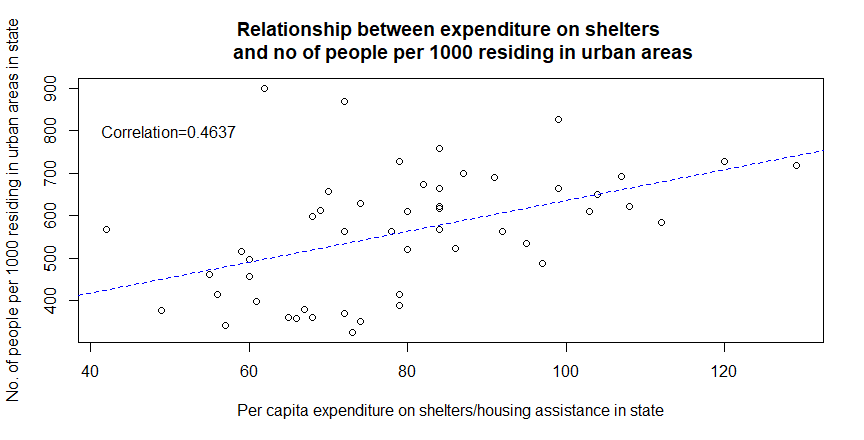
\includegraphics[width=1.3\textwidth]{Y and X3.png}
    \caption{Y and X3}
    \label{fig:enter-label}
\end{figure}

\begin{figure} 
    \centering
    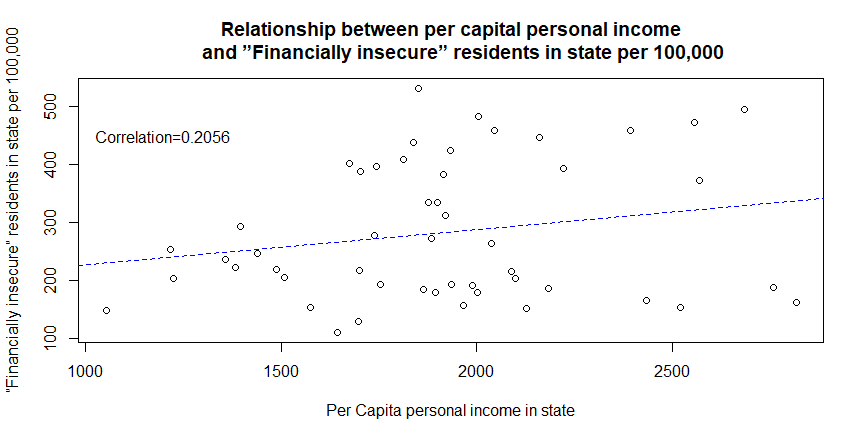
\includegraphics[width=1.3\textwidth]{X1 and X2.png}
    \caption{X1 and X2}
    \label{fig:enter-label}
\end{figure}

\begin{figure} 
    \centering
    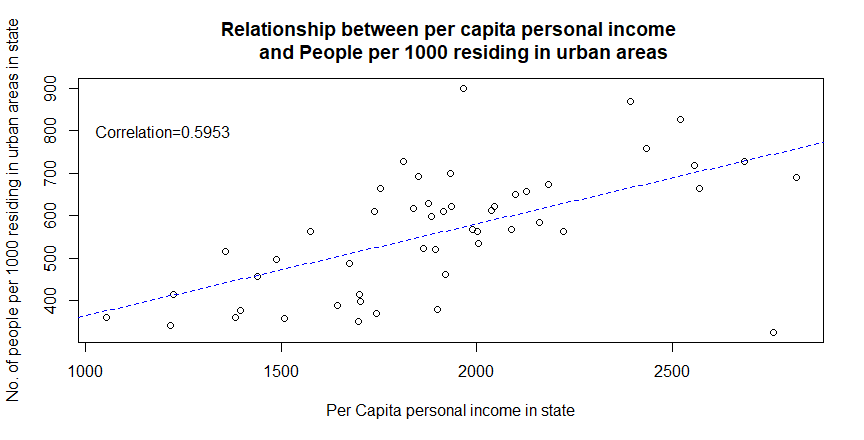
\includegraphics[width=1.3\textwidth]{X1 and X3.png}
    \caption{X1 and X3}
    \label{fig:enter-label}
\end{figure}

\begin{figure} 
    \centering
    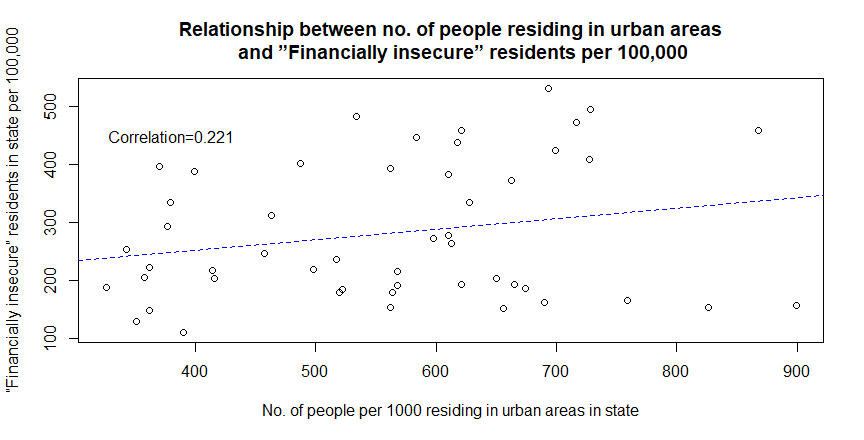
\includegraphics[width=1.3\textwidth]{X2 and X3.png}
    \caption{X2 and X3}
    \label{fig:enter-label}
\end{figure}

\pagebreak
\subsection{Answer 2.2}
Next, I plot the relationship between Y(per capita expenditure on shelters/housing assistance in state) and Region.
For this, I make a boxplot using this code:
\begin{verbatim}
    boxplot(expenditure$Y ~ expenditure$Region,
        main="Boxplot of per capita expenditure on shelters 
        by region",
        ylab="Per capita expenditure on shelters",
        xlab="Region",
        names=c("Northeast","North Central","South","West"))
means <- tapply(expenditure$Y, expenditure$Region, mean)
points(means, pch=20) 
\end{verbatim}

The boxplot (Figure 7) is displayed below.

\noindent The black dots in each boxplot indicate the mean. On the basis of this, I can say that the West (Region 4) has the highest per capita expenditure on housing assistance on average

I also used this code to calculate the mean of the four regions:
\begin{verbatim}
    aggregate(expenditure$Y, list(expenditure$Region), FUN=mean)
\end{verbatim}
This reiterated the same finding that the West had the highest per capita expenditure on housing assistance on average at 88.3.
\begin{table}[]
    \centering
    \begin{tabular}{c|c}
    Region & Mean  \\
    Northeast & 79.44 \\
    North-Central & 83.92 \\
    South & 69.19 \\
    West & 88.31 \\
    \end{tabular}
    \caption{Mean of each region}
    \label{tab:my_label}
\end{table}
\begin{figure}[h]
    \centering
    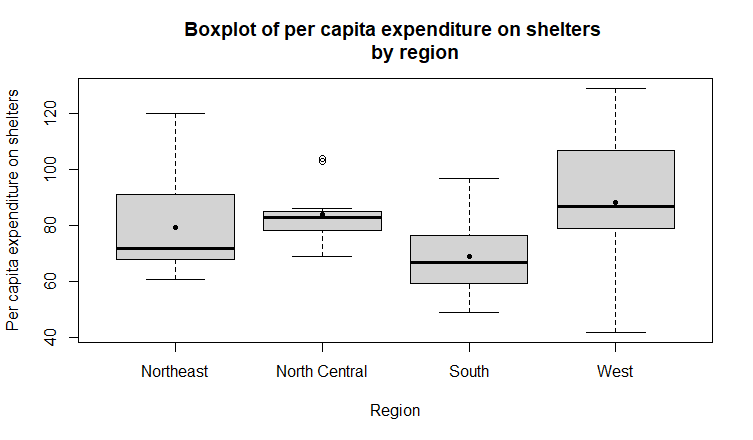
\includegraphics[width=1.4\textwidth]{Y and Region.png}
    \caption{Y and Region}
    \label{fig:enter-label}
    \FloatBarrier
\end{figure}

\pagebreak
\subsection{Answer 2.3}
First, I plot the relationship between Y and X1.

\noindent From the graph below, it is possible to say that there is a moderate positive correlation (0.53) between per capita expenditure on shelters and per capital personal income in the state. 

\begin{figure}[h]
    \centering
    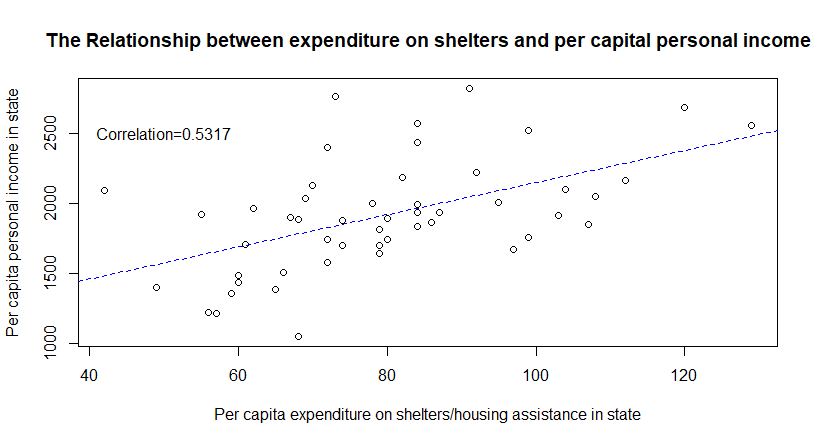
\includegraphics[width=1.3\textwidth]{Y and X1.png}
    \caption{Y and X1}
    \label{fig:enter-label}
\end{figure}

Using this code in R, I added region to the above graph:
\begin{verbatim}
 library(car)
?scatterplot
scatterplot(expenditure$X1 ~ expenditure$Y| 
    expenditure$Region,
    regLine=TRUE,smooth=FALSE, grid=FALSE,
    legend=c(title="Region",coords="topleft"),
    main="The relationship between per capita personal income
    and per capita expenditure on shelters by region",
    xlab="Per capita personal income in state",
    ylab="Per capita expenditure on shelters in state")

\end{verbatim}
\vspace{2cm}

\begin{figure}[h]
    \centering
    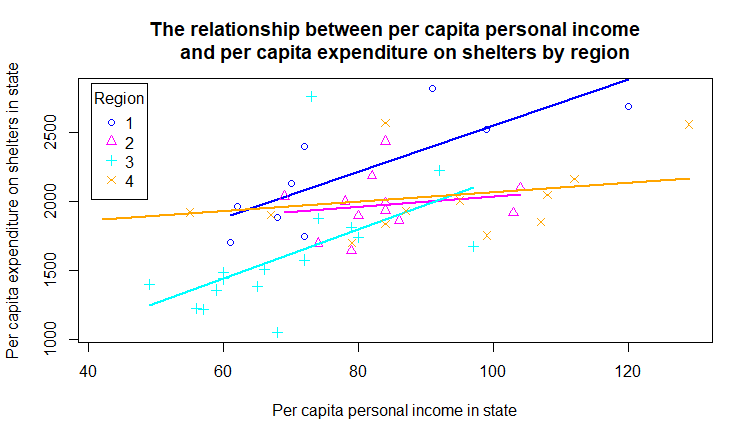
\includegraphics[width=1.4\textwidth]{Y and X1 by Region.png}
    \caption{Y and X1 by region}
    \label{fig:enter-label}
\end{figure}
\vspace{0.7cm}
\noindent On the basis of the graph below, it is possible to make some inferences.

\vspace{0.5cm}
\noindent 

First, Region 1 (Northeast) has the highest per capita expenditure on shelters. Whereas, Region 3 (South) has the lowest per capita expenditure on shelters on average.
\vspace{0.5cm}

\noindent On the basis of the line of best fit, we can say that there is a moderate positive correlation between per capita personal income and per capita expenditure on shelters in Region 1(Northeast) and 3(South). Whereas, there is a weak positive correlation for Region 2(North Central) and 4(West).
The per capital personal income has a large spread for Region 4 (West) which could be a possible explanation for why there is a weak correlation to expenditure on shelters. 

\end{document}
